\setcounter{section}{-1}

\section{基礎}

\subsection{いつものマクロ}

\begin{lstlisting}
#define REP(i,n) for(int i = 0; i < (int)(n); i++)
#define FOR(i,c) for(__typeof((c).begin()) i = (c).begin(); i != (c).end(); ++i)
#define ALLOF(c) (c).begin(), (c).end()
\end{lstlisting}


\subsection{間違ったかな?と思ったら}

\begin{itemize}
\item{\w{とりあえず深呼吸。}}
\item{\w{これフローじゃね?}}
\item{\w{これ二分探索じゃね?}}
\item{\w{これ凸じゃね?}}
\item{\w{最小/最大/特異ケースのテスト}}
\item{-Wall, -Wextraはつけているか?}
\item{問題の条件をよみなおせ!}
\item{入力の形式はあっているか?}
\begin{itemize}
\item{入力ファイルを修正してそのままにしていないか}
\item{スペースを含む文字列}
\item{0-origin, 1-origin}
\item{(i,j) $<$-$>$ (x,y) 変換をはじめとする座標変換}
\item{改行コードwww}
\end{itemize}
\item{出力の形式はあっているか?}
\begin{itemize}
\item{スペルミス}
\item{-0.000}
\item{空行のはさみ方}
\item{デバッグ出力の削りのこし}
\item{解が無い時}
\end{itemize}
\item{オーバーフロー}
\begin{itemize}
\item{答えがintに収まらない}
\item{numeric\_limits$<$int$>$::max() * 2}
\item{bool型の変数にint/doubleを代入、関数の返り値型がbool (特に、DP/メモの型を後で変更した場合)}
\end{itemize}
\item{ポインタの進め忘れ}
\item{参照/イテレータの無効化}
\item{実数}
\begin{itemize}
\item{EPSを使わずに比較していないか}
\item{問題に合ったEPSの設定}
\item{NaN (/, sqrt, asin, acos, etc...)}
\end{itemize}
\item{switch}
\begin{itemize}
\item{breakし忘れていないか}
\item{defaultにassert(false)}
\end{itemize}
\item{ライブラリ関数}
\begin{itemize}
\item{全順序関係でないようなoperator$<$を使ったソート}
\item{accumulate/inner\_productの初期値は必ず型をキャストで明示すること}
\end{itemize}
\item{配列}
\begin{itemize}
\item{サイズは十分か?}
\item{初期化を忘れていないか?}
\item{番兵のせいでサイズ・インデックス・初期化が間違っていないか?}
\item{添字を間違っていないか?(jと書くべきところにi、など)}
\end{itemize}
\item{コピペ}
\begin{itemize}
\item{コピペ修正ミスは無いか?(y += dx みたいな)}
\end{itemize}
\item{考え方}
\begin{itemize}
\item{問題を分解したときに独立にとけないこともあるので柔軟に考えるといいよ}
\end{itemize}
\end{itemize}


%\vfill

%\begin{center}
%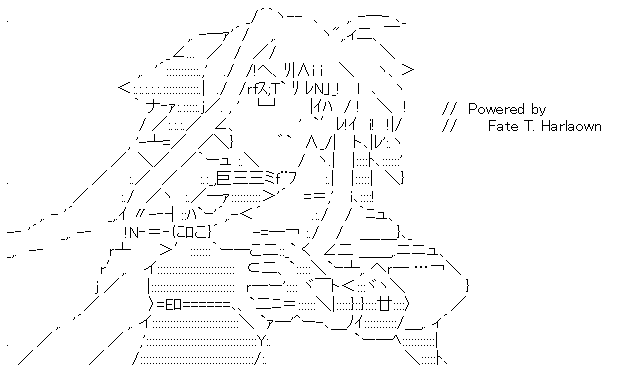
\includegraphics[width=0.98\hsize]{fate2-aa.eps}
%\end{center}

\newpage

